{\color{reviewD}
\presub
\subsection{Extending SS and USS for Other Tasks} %\postsub
\label{eva_other}

\noindent\textbf{Parameter Setting:}
In this subsection, we use Unbiased SS\cite{unbiasedsketch} and SS\cite{spacesaving} to address the other three kinds of tasks.
We use \textit{IP Trace Dataset} to evaluate because only IP Trace Dataset can be used for finding Super-Spreaders.
			
\begin{figure*}[!ht]
	\centering
	\subfigure[CR of Finding \taskfour]{
		\begin{minipage}[t]{0.23\textwidth}{
			\prefig
			\begin{center}
			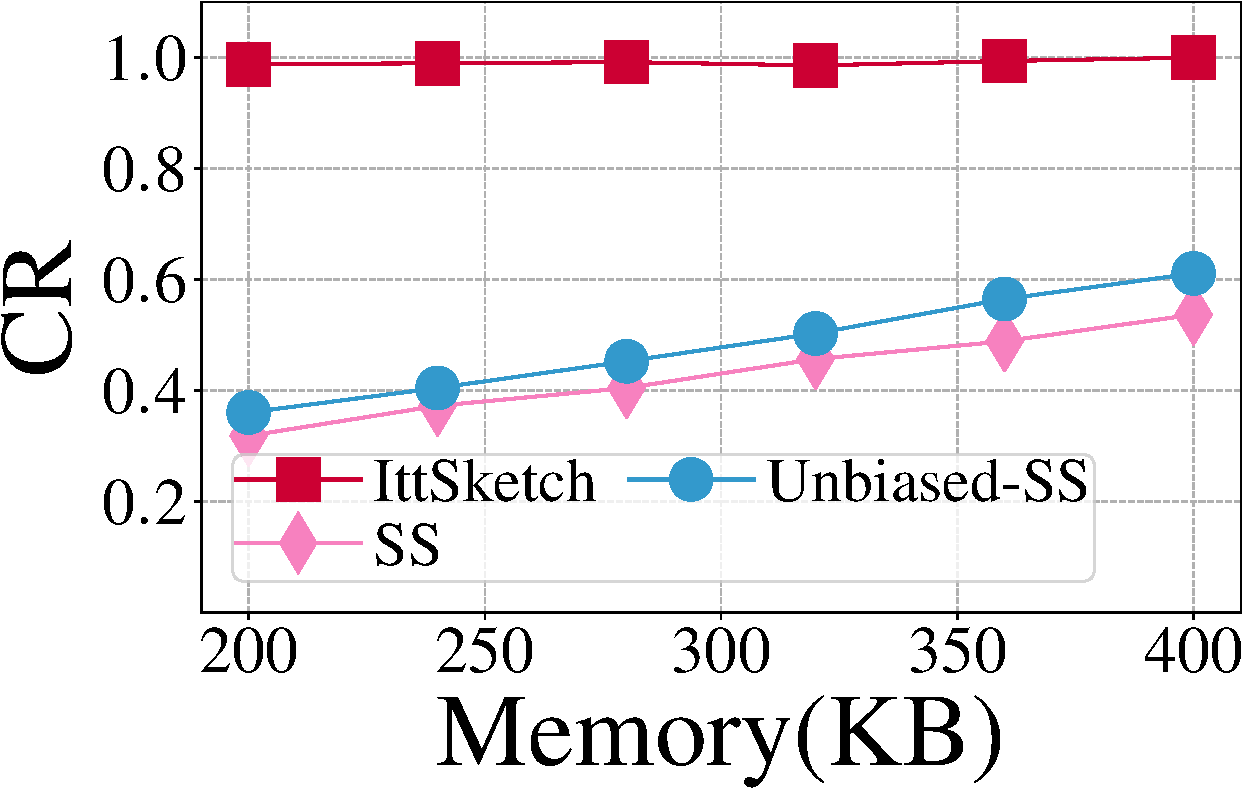
\includegraphics[width=\textwidth, ]{Figures/other/other_cha_cr-cropped.pdf}
			\end{center}}
			\postfig 
			\adjustfigs
			\prefigcaption
			\label{other_cha_cr}
			\postfigcaption
		\end{minipage}
	}
	\subfigure[PR of Finding \taskfour]{
		\begin{minipage}[t]{0.23\textwidth}{
		    \prefig
			\begin{center}
			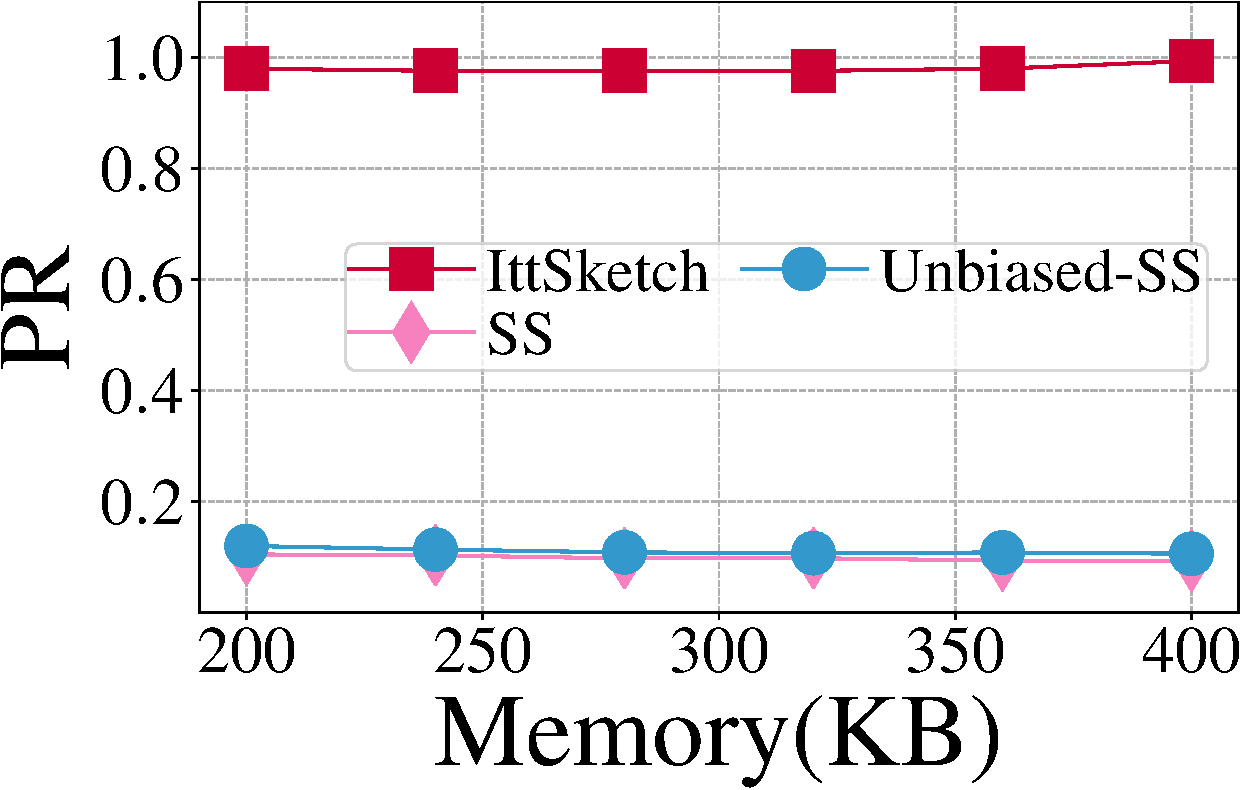
\includegraphics[width=\textwidth, ]{Figures/other/other_cha_pr-cropped.pdf}
			\end{center}}
			\postfig
			\adjustfigs
			\prefigcaption
			\label{other_cha_pr}
			\postfigcaption
		\end{minipage}}
	\subfigure[ARE of Finding \tasktwo]{
		\begin{minipage}[t]{0.23\textwidth}{
			\prefig
			\begin{center}
			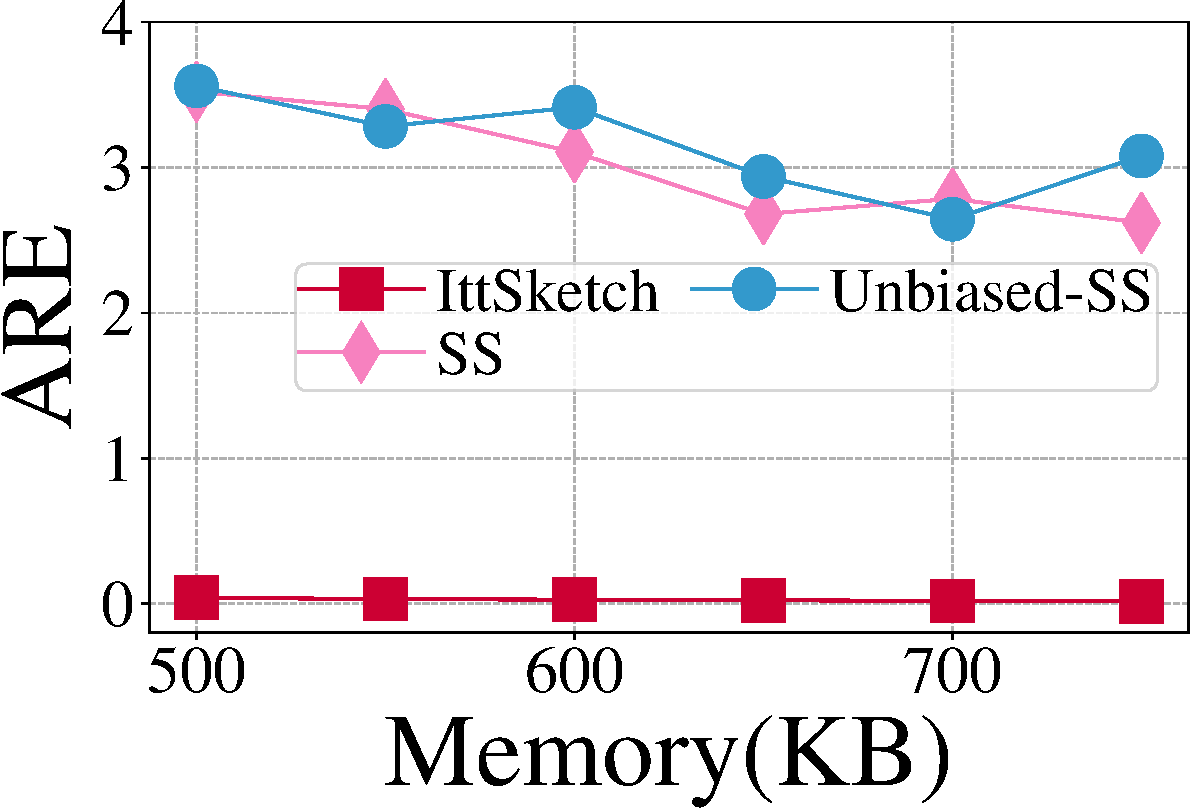
\includegraphics[width=\textwidth, ]{Figures/other/other_sup_are-cropped.pdf}
			\end{center}}
			\postfig 
			\adjustfigs
			\prefigcaption
			\label{other_sup_are}
			\postfigcaption
		\end{minipage}
	}
	\subfigure[ARE of Finding \taskthree]{
		\begin{minipage}[t]{0.23\textwidth}{
		    \prefig
			\begin{center}
			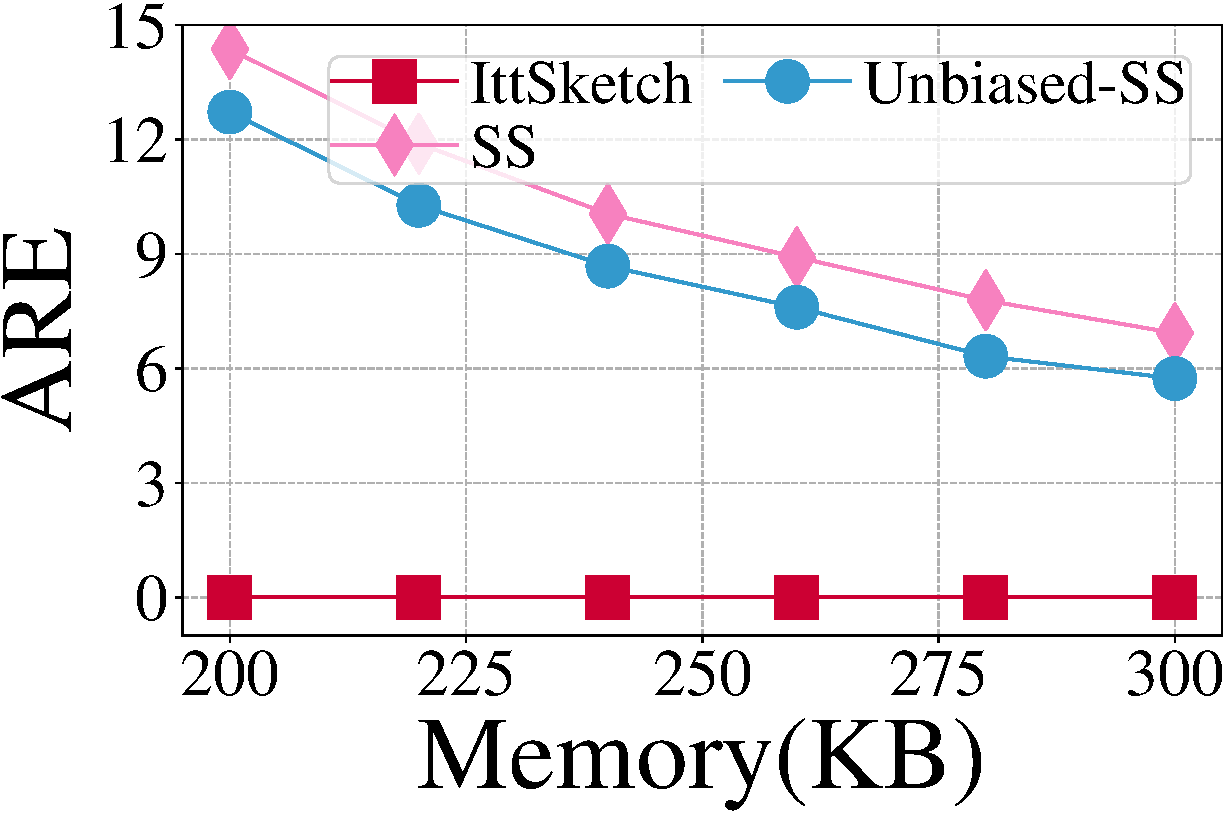
\includegraphics[width=\textwidth, ]{Figures/other/other_per_are-cropped.pdf}
			\end{center}}
			\postfig
			\adjustfigs
			\prefigcaption
			\label{other_per_are}
			\postfigcaption
		\end{minipage}}
	\vvv \vvv
    \caption{Accuracy comparison of InterestSketch, SS, and USS for other three tasks.}
	\label{other}
\end{figure*}

\begin{figure*}[!ht]
	\centering
	\subfigure[Latency of Finding \taskone]{
		\begin{minipage}[t]{0.23\textwidth}{
			\prefig
			\begin{center}
			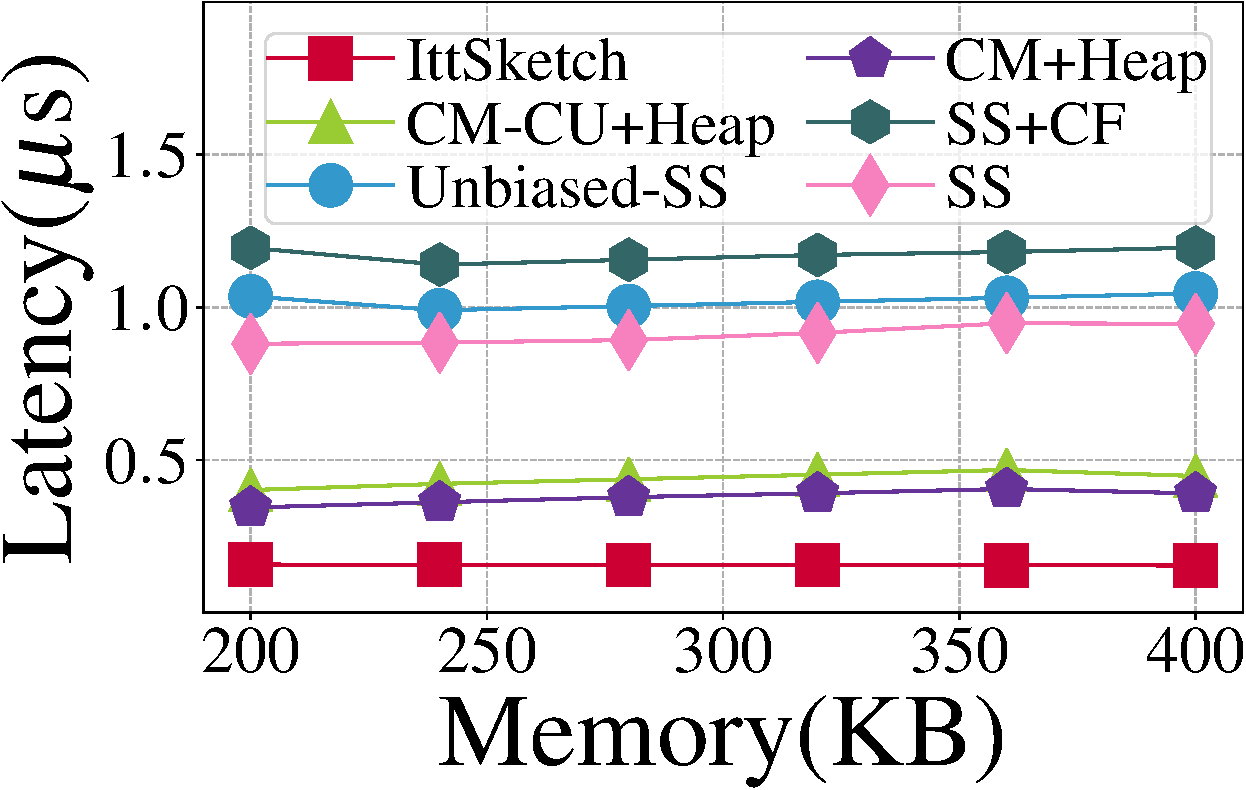
\includegraphics[width=\textwidth, ]{Figures/latency/fre_ip_latency-cropped.pdf}
			\end{center}}
			\postfig 
			\adjustfigs
			\prefigcaption
			\label{fre_ip_latency}
			\postfigcaption
		\end{minipage}
	}
	\subfigure[Latency of Finding \taskfour]{
		\begin{minipage}[t]{0.23\textwidth}{
		    \prefig
			\begin{center}
			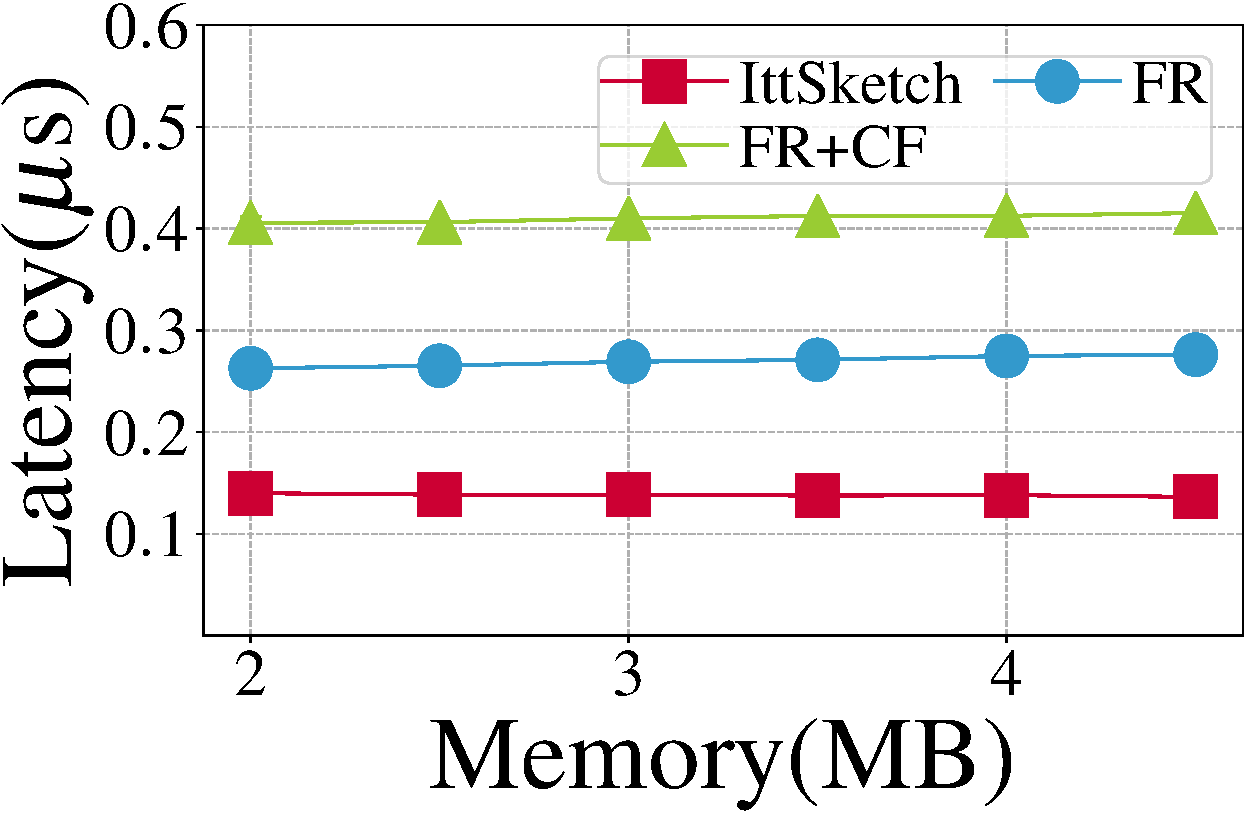
\includegraphics[width=\textwidth, ]{Figures/latency/cha_ip_latency-cropped.pdf}
			\end{center}}
			\postfig
			\adjustfigs
			\prefigcaption
			\label{cha_ip_latency}
			\postfigcaption
		\end{minipage}
	}
	\subfigure[Latency of Finding \tasktwo]{
		\begin{minipage}[t]{0.23\textwidth}{
			\prefig
			\begin{center}
			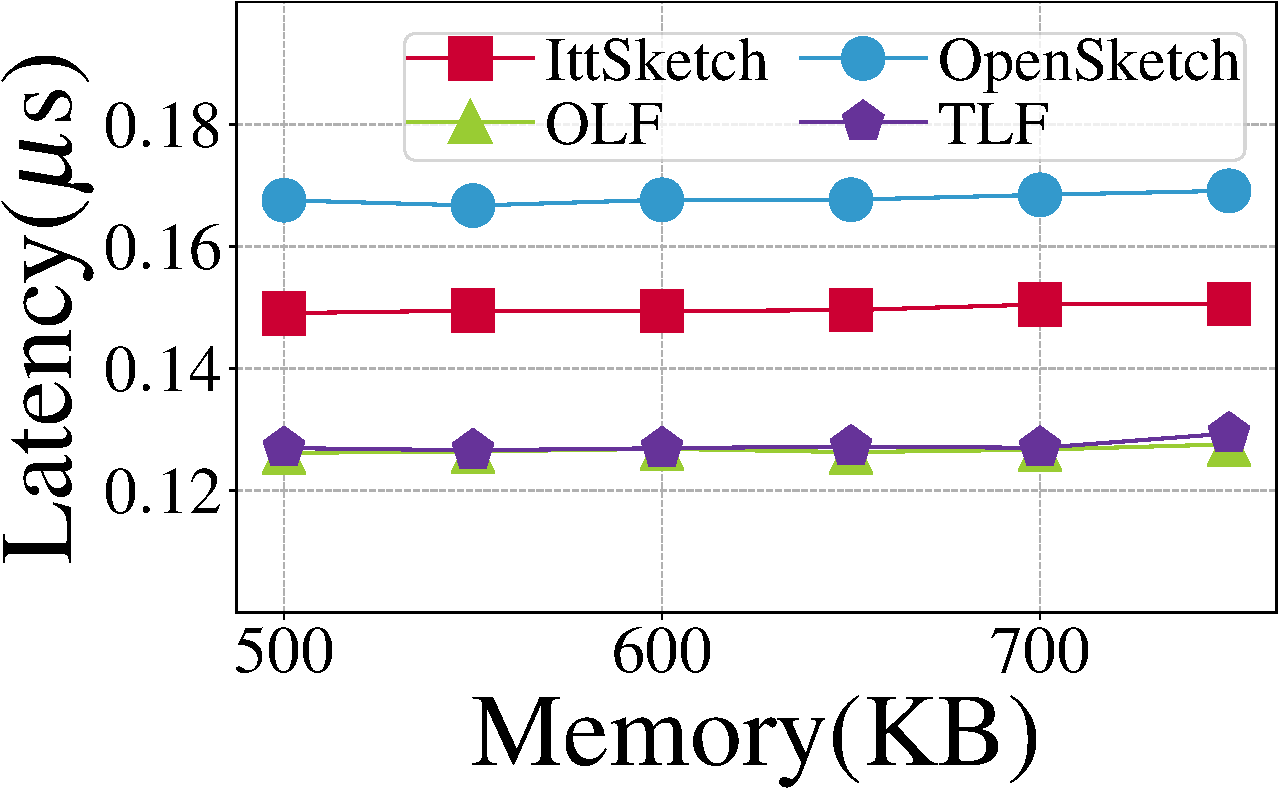
\includegraphics[width=\textwidth, ]{Figures/latency/sup_ip_latency-cropped.pdf}
			\end{center}}
			\postfig 
			\adjustfigs
			\prefigcaption
			\label{sup_ip_latency}
			\postfigcaption
		\end{minipage}
	}
	\subfigure[Latency of Finding \taskthree]{
		\begin{minipage}[t]{0.23\textwidth}{
		    \prefig
			\begin{center}
			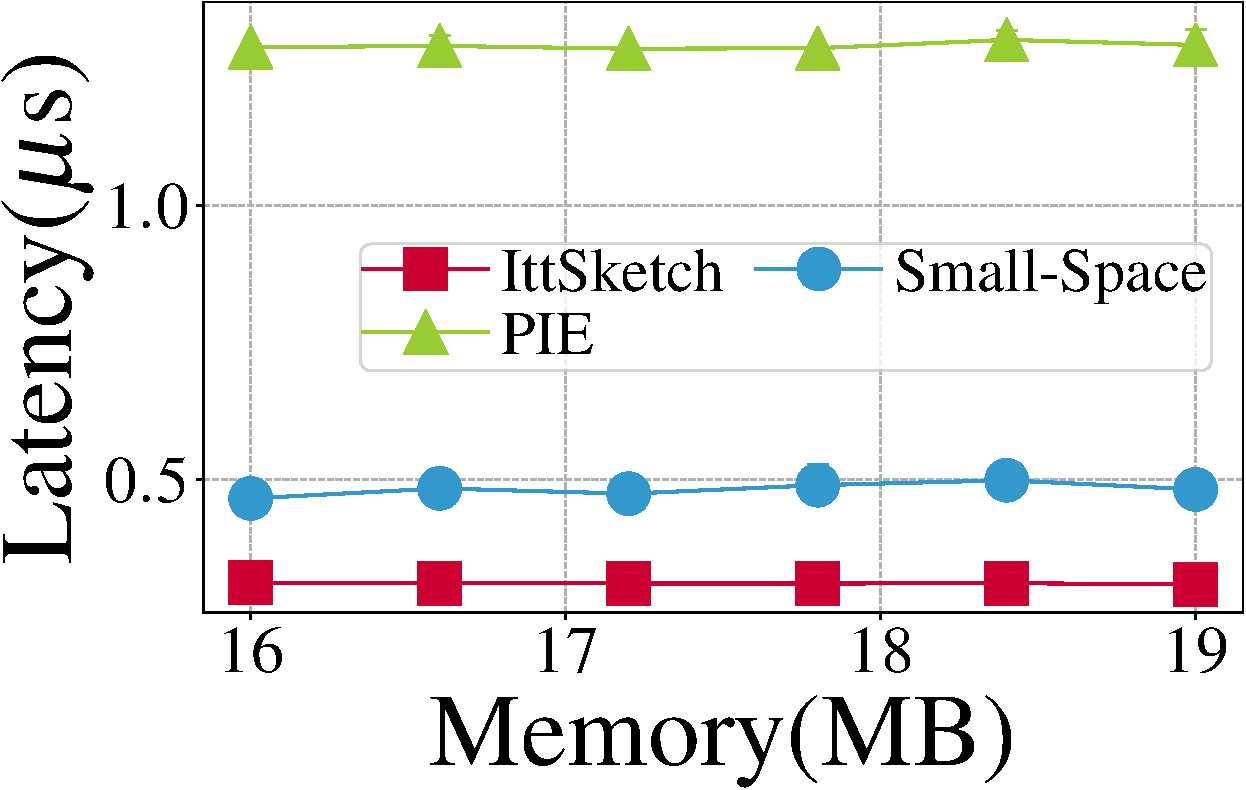
\includegraphics[width=\textwidth, ]{Figures/latency/per_ip_latency-cropped.pdf}
			\end{center}}
			\postfig
			\adjustfigs
			\prefigcaption
			\label{per_ip_latency}
			\postfigcaption
		\end{minipage}
	}
	%\vvv \vvv
    \caption{Latency of four tasks.}
	\label{latency}
\end{figure*}
			
\noindent\textbf{CR and PR of Finding \taskfour{} (Figure~\ref{other_cha_cr}-\ref{other_cha_pr}):}
We can find that, the CR of \sketchname{} is around 2.67 times and 2.45 times higher than SS and Unbiased SS. According to Figure \ref{other_cha_pr}, the PR of \sketchname{} is around 9.33 times and 8.17 times higher than SS and Unbiased SS.

\noindent\textbf{ARE of Finding \tasktwo{} (Figure~\ref{other_sup_are}):}
We find that, the ARE of \sketchname{} is around 115.5 times and 126.7 times higher than SS and Unbiased SS. The ARE of \sketchname{} is often lower than 0.04, while the ARE of SS and Unbiased SS is often higher than 2.6.

\noindent\textbf{ARE of Finding \taskthree{} (Figure~\ref{other_per_are}):}
Our results show that the ARE of \sketchname{} is around 2347 times and 2000 times higher than SS and Unbiased SS. The ARE of \sketchname{} is often lower than 0.006, while the ARE of SS and Unbiased SS is often higher than 5.

\noindent\textbf{Summary:}
%
1) 
The ARE of SS and Unbiased SS are often higher than 2.6.
Similar to the performance on finding frequent items, the ARE of SS and Unbiased SS are often much higher than that of \sketchname{} on other three tasks.
Because they cannot accurately record the frequency of frequent items, they also can not perform well on other tasks which is highly related to item frequencies.
}